\documentclass[letterpaper, 10pt, onecolumn, draftclsnofoot]{IEEEtran}

%Packages
\usepackage{cite}
\usepackage{graphicx}
\usepackage{amssymb}                                         
\usepackage{amsmath}                                         
\usepackage{amsthm}
\usepackage{alltt}                                           
\usepackage{float}
\usepackage{url}
\usepackage{balance}
\usepackage[margin=0.75in]{geometry}
\usepackage{listings}
\usepackage{color}
\usepackage{textcomp}

\usepackage{hyperref}
\hypersetup{
    colorlinks=true,
    linkcolor=black,
    filecolor=black,      
    urlcolor=black,
}

\lstset{
	tabsize=5,
	rulecolor=,
	language=matlab,
        basicstyle=\scriptsize,
        upquote=true,
        aboveskip={0.5\baselineskip},
        columns=fixed,
        showstringspaces=false,
        extendedchars=true,
        breaklines=true,
        prebreak = \raisebox{0ex}[0ex][0ex]{\ensuremath{\hookleftarrow}},
        frame=L,
        showtabs=false,
        showspaces=false,
        showstringspaces=false,
        identifierstyle=\ttfamily,
        keywordstyle=\color[rgb]{0,0,1},
        commentstyle=\color[rgb]{0.133,0.545,0.133},
        stringstyle=\color[rgb]{0.627,0.126,0.941},
}

\title{CS 444 \\ Spring 2018  \\ Final Paper}
\author{Zachary Thomas}
\date{April 29th, 2018}

\begin{document}
	\begin{titlepage}
		\maketitle
	\end{titlepage}
\newpage
\tableofcontents
\newpage

\section{Introduction}

This document covers fundamental operating system concepts for three different operating systems. The three operating systems we are interested in are Windows, FreeBSD, and Linux. Throughout this document Windows and FreeBSD will be compared to Linux. The main topics covered are process, threads, CPU scheduling, I/O, provided functionality, file systems, and VFS.

\section{Windows and Linux Processes, threads, and CPU scheduling comparison}

Windows NT is a hybrid kernel, Its microkernel features allow many of its components to be swapped out, the main drawback is that this also leads to higher overhead and worse performance than pure monolithic systems such as Linux.\cite{wi_srv}

\subsection{Processes}

In Windows a processes is an instance of a program that is being executed. One of the methods for Windows to create a process is to run the CreateProcess function, this function performs the following steps to create a new process.\cite{wi_p1}

\subsubsection{Converting and validating parameters and flags}

Here the priority of the new process is set. If no priority is selected then it defaults to normal.\cite{wi_p1}

\subsubsection{Opening the Image to Be Executed}

At this point the system attempts to find the correct Windows image file to run the file given by the caller. The system considers many possible options based on information it is given about the file, for POSIX it will run Posix.exe, for Win16 it will run Ntvdm.exe, etc.. If the system can not find a file to run CreateProcess will fail.\cite{wi_p1}

\subsubsection{Creating the Windows Executive Process Object}

Now that a Windows executable file has been opened Windows creates an executive process object. The process object stores important values such as parent process ID and it initializes the address space of the process.\cite{wi_p1}

\subsubsection{Creating the Initial Thread and Its Stack and Context}

We now have a ready processes but without any threads it can not begin execution. Two routines by the name of PspAllocateThread and PspInsertThread create our first thread in this stage.\cite{wi_p1}

\subsubsection{Performing Windows Subsystem–Specific Post-Initialization}

At this point all executive process and thread objects have been created.  
In this stage Windows does a number of checks to determine if this executable will be allowed to run as well as finish initializing the process.\cite{wi_p1} 

\subsubsection{Starting Execution of the Initial Thread}

Put simply the processes initial thread starts running. \cite{wi_p1} 

\subsubsection{Performing Process Initialization in the Context of the
New Process}

At this point the initial thread is running in kernel mode, it runs a startup routine and an initial thread routine. It does a number of checks, such as seeing if it is a debugger and should be launched in debug mode. Once it has completed all checks it returns to user mode, at this point the thread execution begins.\cite{wi_p1}

Windows systems creates processes in a very different way than Linux systems. Notably creating a thread is an essential part of Windows process creation. Linux on the other hand does not require any threads for a process to function. 

Additionally for a Linux system we expect most processes to be created by using fork() to create a child process that is a duplicate of the parent and then exec() to load a new executable into  the address space that is then used.
Another major distinction between Windows and Linux's process handling is how child process are dealt with once a parent process has terminated. When a parent process dies in Linux the init process (the process that started when the system was booted) will adopt the orphan process and then kill it. Windows on the other hand does not terminate child processes when a parent process is terminated. Child processes are simply allowed to remain.\cite{wi_p1, linux}

\begin{figure}[!ht]
  \caption{The main stages of process creation in Windows\cite{wi_p1}}
  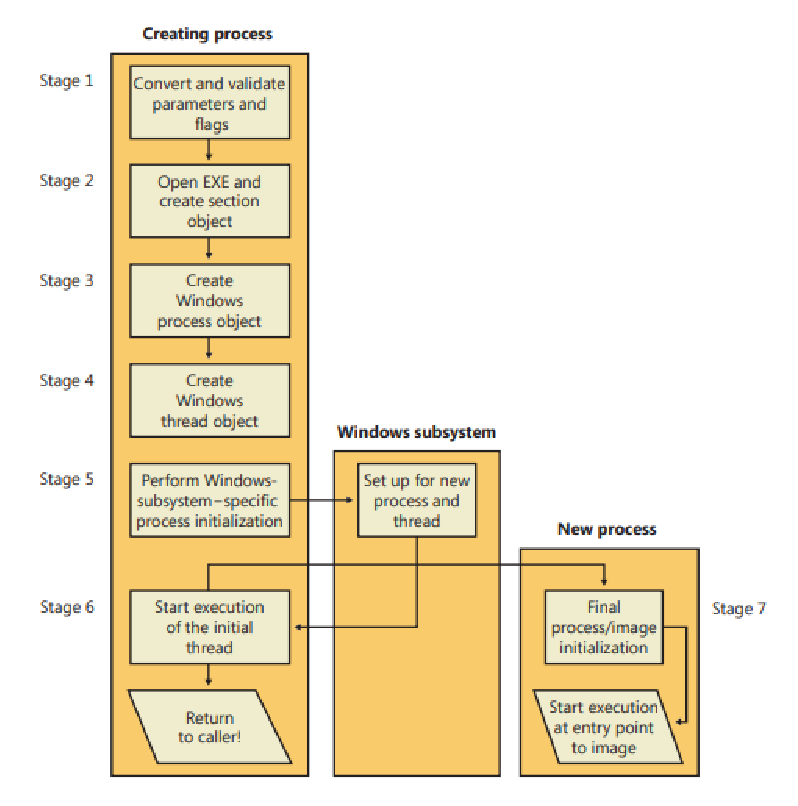
\includegraphics[scale=0.75]{wpd.eps}
\end{figure}

\subsection{Threads}

In Windows a process is like a container that must always be holding at least one thread, these threads themselves are the units of execution, without them a processes can not function. This is in contrast to a Linux system in which threads and processes are identical with the exception that Linux threads share certain resources with other processes.\cite{wi_p1}

Threads in Windows contain a stack for user space and a stack for kernel space execution. This is to help facilitate threads being able to switch back and forth from user and kernel space. For a thread to enter kernel space something must initiate the switch such as making a system call. The processor then issues an instruction that switches the calling thread to kernel space. Once the system service is finished the thread is returned to user space.\cite{wi_p1}

It is also worth mentioning that each thread shares its processes virtual memory space, this means that these threads can all read and write to their processes virtual memory, but generally can not write or read the memory of other processes.\cite{wi_p1}

\subsection{CPU Scheduling}

Windows has two processor access modes. The first is user mode which handles processes that a user would run, such as a web browser, or a word processor. The second is kernel mode it handles trusted processes, such as system services and device drivers. Only kernel mode gets full access to all memory and CPU instructions. Linux systems also use a user and kernel mode as it helps limit the damage a user or unreliable software can do to the system.\cite{wi_p1}

Windows does not use a single scheduler module, but rather has scheduling events spread across the kernel. The following events can trigger the system to make scheduling decisions: A thread becomes ready to execute, a thread leaves the running state, a thread's priority changes, or a thread's processor affinity changes switching the processor it runs on. One important distinction to make is that only threads are considered when scheduling, processes are ignored.\cite{wi_p1} 

This means if only two processes are running and they have threads with the same priority, if one process has a single thread and the other has nine, the process with a single thread will only get one tenth of the CPU time. This is somewhat similar to Linux's completely fair scheduler. The CFS focuses on fairness, but since Linux does not differentiate between threads and processes as far as scheduling is concerned, we would see a process with many threads getting much more CPU time than one with a single thread.\cite{linux,wi_p1}

\section{FreeBSD and Linux Processes, threads, and CPU scheduling comparison}

FreeBSD is one of the first open source operating systems, since it is a direct descendant of genuine UNIX we can reason that FreeBSD has closer roots to UNIX than Linux does. It is also worth noting that FreeBSD and Linux both use a monolithic kernel, meaning that the entirety of these operating systems are working in kernel space.\cite{BSD_ORG}

\subsection{Processes}

In FreeBSD processes are programs in execution and each must contain at least one thread. There are two ways in which a process is created. The first scenario is during startup where a single process is crafted by the kernel. The second scenario is when processes are created by the kernel duplicating another process, this new process is known as a child process while the original process is known as a parent process. To manage this actual duplication the system call fork is used, it copies the parent processes and it shares the same resources. At this point the child is simply the same process as the parent. To run a different process the next step is for the child to use the system call execve which executes the program pointed to by a given filename, Now we have a child that is no longer a copy of the parent. When this child eventually terminates it becomes what is known as a zombie process. Zombies processes simply wait for their parent process to clean them up. A parent may use the wait system call to collect the process id of the zombie and its exit status, at this point the zombie gets removed from the system. If the parent process exits before the child process is cleaned up then the kernel arranges the steps needed to remove it.\cite{BSD}

It is worth noting that FreeBSD and Linux create processes in a very similar manner, such as both using a fork and execute system call, and not allowing child process to remain without a parent. Unlike freeBSD however Linux does not require a thread for a process to function as Linux can use a thread-less process to perform execution.\cite{linux,BSD}

\lstset{language=C,caption={FreeBSD's fork.c \cite{code1}},label=code1}
\begin{lstlisting}[language=C]
#include <sys/cdefs.h>
__FBSDID("$FreeBSD$");

#include <sys/types.h>
#include <unistd.h>
#include "libc_private.h"

__weak_reference(__sys_fork, __fork);

#pragma weak fork
pid_t
fork(void)
{

	return (((pid_t (*)(void))__libc_interposing[INTERPOS_fork])());
}
\end{lstlisting}

\subsection{Threads}

In FreeBSD all threads that are in a runnable state are assigned a priority in a run queue. It is easiest to think of processes as containers for threads, where each container must house at least one thread. The threads themselves are the units of execution. In addition each user thread also has an equivalent kernel thread that acts on its behalf in kernel space when dealing with system calls, page faults, or signal deliveries.\cite{BSD}

Threads in FreeBSD are implemented as part of a process while in Linux threads are the same thing as processes with the exception of sharing certain resources with other processes.\cite{linux, BSD}

\subsection{CPU Scheduling}

Scheduling in FreeBSD is done with the ULE scheduler and is split into two parts a low-level scheduler and a high-level scheduler. The low-level scheduler runs thousands of times a second, this scheduler waits until a thread blocks and then grabs the next highest priority thread to run from a set of run queues, if there are multiple threads in the queue it has selected, then the threads in that queue get run in a round robin fashion with each getting an equal amount of time. The high-level scheduler runs up to a few times per second, its job is to organize threads by priority into a specific run queue on a specific CPU. Each CPU gets its own set of run queues this is to prevent conflict from arising as two CPUs may try to run the same thread if their last running thread stopped at the same time.\cite{BSD}

While Linux's completely fair scheduler does use a similar priority-based scheduling as FreeBSD's ULE scheduler which attempts to have high priority processes/threads run before lower priority processes/threads, it does not use run queues. Linux also offers support for many schedulers beyond CFS, FreeBSD reduces overhead by requiring the scheduler to be set at the time that the kerenl is built. In addition CFS focuses on giving each process an equal time slice by dividing the time slice across the number of processes, one notable difference is that unlike CFS, ULE favors interactive processes at the cost of fairness.\cite{BSD, linux, jeff}

\lstset{language=C,caption={FreeBSD's sched\_ule.c\cite{code2}},label=code2}
\begin{lstlisting}[language=C]
 * These macros determine priorities for non-interactive threads.  They are
 * assigned a priority based on their recent cpu utilization as expressed
 * by the ratio of ticks to the tick total.  NHALF priorities at the start
 * and end of the MIN to MAX timeshare range are only reachable with negative
 * or positive nice respectively.
 *
 * PRI_RANGE:	Priority range for utilization dependent priorities.
 * PRI_NRESV:	Number of nice values.
 * PRI_TICKS:	Compute a priority in PRI_RANGE from the ticks count and total.
 * PRI_NICE:	Determines the part of the priority inherited from nice.
 */
#define	SCHED_PRI_NRESV		(PRIO_MAX - PRIO_MIN)
#define	SCHED_PRI_NHALF		(SCHED_PRI_NRESV / 2)
#define	SCHED_PRI_MIN		(PRI_MIN_BATCH + SCHED_PRI_NHALF)
#define	SCHED_PRI_MAX		(PRI_MAX_BATCH - SCHED_PRI_NHALF)
#define	SCHED_PRI_RANGE		(SCHED_PRI_MAX - SCHED_PRI_MIN + 1)
#define	SCHED_PRI_TICKS(ts)						
    (SCHED_TICK_HZ((ts)) /						
    (roundup(SCHED_TICK_TOTAL((ts)), SCHED_PRI_RANGE) / SCHED_PRI_RANGE))
#define	SCHED_PRI_NICE(nice)	(nice)
\end{lstlisting}

Another similarity that FreeBSD and Linux share is the use of nice values, as the above code shows a nice value helps determine the priority of a process. Higher nice values imply that the process is being nice and letting other processes go first and have more time. A thread with a low nice value means that it is a high priority thread and should be ran first and/or given a larger time slice.\cite{BSD}

\section{Windows and Linux I/O and provided functionality comparison}

\subsection{I/O management}
Windows represents I/O by using something called a I/O request packet (IRP). When a process needs to use an I/O device the I/O manager creates an IRP and sends it to the relevant driver. Once the requested I/O operation is completed the I/O manager removes the associated IRP. When drivers receive these requests they perform the requested operation and then return the request to the I/O manager. To reduce the complexity of drivers the I/O manager also has number of functions that can be called by drivers, these functions may be used by many drivers so it reduces the need for drivers to contain extra code.\cite{wi_p2}
To prioritize I/O windows uses the I/O manager to split I/O into five categories of priority: critical, high, normal, low, and very low (high and low are typically not used). Background processes such as a virus scan are given very low priority so that they do not negatively affect other I/O.
Next a set of queues are assigned based on priority and another set of queues are assigned based on if an I/O is idle or not. I/O that is not idle is given priority over idle I/O, and critical I/O is given priority over normal I/O. To prevent idle I/O from never getting processed the system guarantees at least one I/O processed approximately every half second.\cite{wi_p2}

In contrast to Windows Linux uses a scheduler that focuses on processes and fairness. By default Linux uses the Completely Fair Queuing I/O scheduler, which divides up I/O requests into queues based on its process of origin, these queues are then sorted sector wise. After all queues are sorted the scheduler services them in a round robin fashion.\cite{linux}

\begin{figure}[H]
  \caption{Sample entries in a global I/O queue in Windows\cite{wi_p2}}
  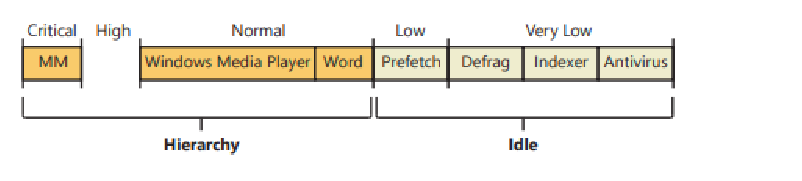
\includegraphics[scale=1]{qd.eps}
\end{figure}

\subsection{Device Drivers}

In Windows all device drivers are either user-mode or kernel-mode drivers. WDM drivers are kernel-mode drivers that can be split into the following three categories:\cite{wi_p2}

\subsubsection{Bus drivers}
Bus drivers detect devices connected to a bus, as well as manage power for that bus.\cite{wi_p2}

\subsubsection{Function drivers}
Function drivers allow the operating system to interface with a given device.\cite{wi_p2}

\subsubsection{Filter drivers}
Filter drivers sit between drivers such as the bus and function drivers and manipulate the behavior of other drivers and devices.\cite{wi_p2}

Hardware often requires a number of layered drivers to allow the hardware as a whole to behave as desired, here is a list of some additional drivers:\cite{wi_p2}

\subsubsection{Class drivers}
Class drivers handle the I/O of a standardized device for which I/O is standardized across differing brands, such as DVD, or CD-ROM.\cite{wi_p2}

\subsubsection{Miniclass drivers}
Miniclass drivers are similar to class drivers but are more specialized, they do not use IRP and rather are kernel-mode DLLs. 
Miniclass drivers are ideal for a device that differs between brands enough to warrant its own drivers.\cite{wi_p2}

\subsubsection{Port drivers}
Port drivers are kernel-mode libraries of functions that relate to a specific type of I/O port. Microsoft writes most port drivers.\cite{wi_p2}

\subsubsection{Miniport drivers}
Miniport drivers are similar to port drivers but are more specialized, they do not use IRP and rather are kernel-mode DLLs. They map I/O to an adapter from a port. These are mostly written by third parties.\cite{wi_p2}

Linux does not offer layered drivers, instead Linux implements drivers as kernel modules. Most devices in Linux are either block devices, such as a hard disk drive with random access memory, or they are character devices where there is a stream of bytes that are consumed when read.\cite{Linux_driver,wi_p2}

\subsection{I/O synchronization}
By default Windows I/O operations are synchronous. Synchronous operations cause the caller to wait for the I/O operation to complete before they continue execution. Asynchronous I/O operations on the other hand can be called and run in parallel with the caller, returning whenever they have completed. To use asynchronous I/O operations the FILE\textunderscore FLAG\textunderscore OVERLAPPED flag must be set when the Createfile function is called.\cite{wi_p2}

Linux also uses synchronous and asynchronous I/O operations, and like Windows it defaults to synchronous operations. Unlike Windows Linux performs specific system calls such as aio\textunderscore read and aio\textunderscore write to create asynchronous I/O operations, instead of simply setting a flag.\cite{linux} 

\subsection{Data structures}
While windows supports many different data structures I will be focusing on lists.

\subsubsection{Singly-linked list}
Singly-linked lists have a head and any number of elements.
Both the elements and the head are represented by the SINGLE\_ LIST\_ ENTRY structure. SINGLE\_ LIST\_ ENTRY contain a Next member, this member points to the next element in the list. The head's Next member points to the first entry in the list. Singly-linked lists in Windows are NULL terminated. Singly-linked lists can only be traversed in one direction.\cite{windows-driver-content}

\subsubsection{Doubly-linked list}
Doubly-linked lists have a head and any number of elements.
Both the elements and the head are represented by the LIST\_ ENTRY structure. LIST\_ ENTRY contain a Flink member and a Blink member these are pointers to other LIST\_ ENTRY structures. Flink points to the next entry in the list, if there are no more entries Flink will point to the head of the list. Blink points to the previous entry in the list, if it is the head it points to the end of the list. Doubly-linked lists in Windows are circular. Doubly-linked lists can be traversed in either direction.\cite{windows-driver-content}

Linux and Windows both implement circular doubly-linked lists by default. This is most likely to make it easier to add and remove elements in the list.\cite{linux}

Linux handles lists of structures differently than in Windows. In Windows we might turn a structure into a linked list, Linux instead will embed a linked list node in the structure.\cite{linux}

\section{FreeBSD and Linux I/O and provided functionality comparison}

\subsection{I/O management}
I/O management in FreeBSD is done via descriptors for all user  processes. These descriptors help classify the object being referenced, for example the VNODE descriptor lets the OS know that it is dealing with a file or device and is created by means of the open system call, while the FIFO descriptor lets the OS know that it is dealing with a named pipe and is created by means of the pipe system call.\cite{BSD}

The default FreeBSD scheduler is C-LOOK. C-LOOK sorts requests based on their distance from the read/write head. All requests above the current sector that the head is currently in are next in the queue, while all request below are handled on the next acceding pass. C-LOOK never descended through the queue, instead it simply restarts at the beginning once it reaches the end.\cite{BSD_hybrid}

FreeBSDs scheduler focuses on throughput while Linux's CFQ scheduler focuses on fair scheduling. The default scheduler for Linux is the Completely Fair Queuing I/O scheduler, which divides up I/O requests into queues based on its process of origin, these queues are then sorted sector wise. After all queues are sorted the scheduler services them in a round robin fashion.\cite{linux} 

\subsection{Device Drivers}
In FreeBSD a device driver can be divided into four parts:\cite{BSD}

\subsubsection{Autoconfiguration and initialization routines}
This part of the driver is called when a device is first connected. It probes and confirms that the device is connected and initializes it.\cite{BSD}

\subsubsection{Routines for servicing I/O requests}
The code that makes up routines for servicing I/O requests is known as the top half of a device driver. Routines for servicing I/O requests handle incoming I/O requests from system calls or from the virtual-memory system.\cite{BSD}

\subsubsection{Interrupt service routines}
The code that makes up interrupt service routines is known as the bottom half of a device driver. The interrupt service routines are called when a device causes an interrupt.\cite{BSD}

\subsubsection{crash-dump routine}
Not all device drivers have a crash-dump routine. Crash-dump routines are called when the system realizes a crash is about to happen and the crash-dump routine records the contents of physical memory for later review.\cite{BSD}

Both Linux and FreeBSD recognize devices as character devices, which act as a stream of bytes that are removed as they are read. In addition they both recognize block devices which are random access, block addressable, such as a hard disk drive.\cite{linux} 

\subsection{I/O synchronization}
Default behavior for FreeBSD is to use synchronous I/O operations. FreeBSD did not always have asynchronous I/O operations, circa 1993 asynchronous I/O interfacing was added to FreeBSD.\cite{BSD}

When a process wishes to use an asynchronous I/O operation it uses the aio\textunderscore read call for reading and the aio\textunderscore write call for writing. If a process gets to a point where it must access data from an asynchronous I/O operation it can use the aio\textunderscore suspend call to wait for completion of the operation, and then it can use the aio\textunderscore return call to return the value from the asynchronous request.\cite{BSD}

\lstset{language=C,caption={FreeBSD's aio\_read and aio\_write.\cite{code3}},label=code3}
\begin{lstlisting}[language=C]
int
__aio_read(struct aiocb *iocb)
{

	return aio_io(iocb, &__sys_aio_read);
}

int
__aio_write(struct aiocb *iocb)
{

	return aio_io(iocb, &__sys_aio_write);
}
\end{lstlisting}

Linux also uses synchronous and asynchronous I/O operations, including some of the same calls that FreeBSD use, such as aio\_read and aio\_write.\cite{linux}

\lstset{language=C,caption={Linux's aio\_read and aio\_write.\cite{code4}},label=code4}
\begin{lstlisting}[language=C]
	switch (type) {
	case AIO_READ:
		iocbp->aio_lio_opcode = IOCB_CMD_PREAD;
		break;
	case AIO_WRITE:
		iocbp->aio_lio_opcode = IOCB_CMD_PWRITE;
		break;
	case AIO_MMAP:
		iocbp->aio_lio_opcode = IOCB_CMD_PREAD;
		iocbp->aio_buf = (unsigned long) &c;
		iocbp->aio_nbytes = sizeof(c);
		break;
	default:
		printk(UM_KERN_ERR "Bogus op in do_aio - %d\n", type);
		return -EINVAL;
	}
\end{lstlisting}

\subsection{Data structures}
We will start with a handful of the data structures that are available in FreeBSD. Within the queue.h file four separate data structures are defined:
\subsubsection{Singly-linked list}
Each list is headed by a forward pointer. Each element is linked to the next in a forward direction. These means that the list can only be traversed in a forward direction.\cite{queue_h}
\subsubsection{Singly-linked tail queue}
There are two pointers, one to the head of the list and one to the tail of the list. The elements with in are linked in a forward direction, meaning that the list can only be traversed in a forward direction.\cite{queue_h}
\subsubsection{List}
Each list is headed by a forward pointer. Each element in the list is linked in both directions. These lists can be traversed in either direction.\cite{queue_h}
\subsubsection{Tail queue}
There are two pointers, one to the head of the list and one to the tail of the list. Each element in the list is linked in both directions. These lists can be traversed in either direction.\cite{queue_h}

In FreeBSD lists are NULL terminated, but in Linux by default lists are circular. This allows looping through the contents of a linked list with the added risk of iterating in a infinite loop (a function such as list\_ for\_ each\_ entry prevents the risk of an infinite loop).\cite{linux}

Linux handles lists of structures differently than FreeBSD. In FreeBSD we might turn a structure into a linked list, Linux instead will embed a linked list node in the structure.\cite{linux}

\lstset{language=C,caption={FreeBSD's Tail queue declaration.\cite{code5}},label=code5}
\begin{lstlisting}[language=C]
#define	TAILQ_HEAD(name, type)						
struct name {								
	struct type *tqh_first;	/* first element */			
	struct type **tqh_last;	/* addr of last next element */		
	TRACEBUF							
}

#define	TAILQ_CLASS_HEAD(name, type)					
struct name {								
	class type *tqh_first;	/* first element */			
	class type **tqh_last;	/* addr of last next element */		
	TRACEBUF							
}

#define	TAILQ_HEAD_INITIALIZER(head)					
	{ NULL, &(head).tqh_first, TRACEBUF_INITIALIZER }
\end{lstlisting}

\section{Windows and Linux File systems and VFS comparison}

\subsection{CDFS and UDF}

Windows offers the CDFS file system as a read-only file system used for CD-ROM. Though this file system is outdated when compared to UDF (Universal disk format) which has become the standard and offers read/write support for Blue-ray, DVD, and more.\cite{wi_p2}

Linux does support UDF, meaning that contents on a DVD using the UDF file system can be shared between Windows and Linux computers.\cite{linux}

\subsection{FAT12, FAT16, FAT32, and exFAT}

Fat12 uses a 12-bit cluster, Fat16 uses 16-bit cluster, and Fat32 uses a 32-bit cluster. These file systems are compatible with most operating systems which makes them ideal if you plan to share files across multiple operating systems, this is why flash drives tend to use either FAT32 or exFAT as their file system. If you plan to use only Windows when accessing your files it might be better to consider using NTFS instead as it is newer and offers more features than the FAT file systems.\cite{wi_p2}

Everything considered it should come as no surprise that Linux supports the FAT file systems. Similar to Windows, if the user never intends to transfer their files across operating systems the FAT file systems are out classed by many of Linux's available file systems, such as Ext4 and ReiserFS.\cite{linux}

\subsection{NTFS}

NTFS is Windows native file system. NTFS uses 64-bit cluster numbers and volumes are limited to just under 256 TB. NTFS was designed to minimize data loss due to unexpected shutdown and offers integrated security.\cite{wi_p2}

To minimize the damage done from a sudden crash NTFS uses atomic transaction. This means that once a transaction of data has started if it is interrupted it will revert to a previously stable state before the transaction started. Additionally NTFS keeps redundant vital file system information in the case of corruption or damage. Users can also take advantage of data redundancy via the volume manager which can duplicate data across multiple disks.\cite{wi_p2}

NTFS also supports sparse files. Consider a 1 GB file that has 10 MB of actual data and the rest of it is empty. If the file is marked as sparse only the 10 MB are actually written to the volume and the empty space is represented as zero filled.\cite{wi_p2}

It is worth noting that while NTFS is a file system designed for Windows and developed by Microsoft, NTFS is useable on Linux systems.\cite{linux}

When comparing NTFS to Linux's Ext4 there are a few notable differences. First more characters are allowed in a filename for the Ext4 file system. Characters such as ":", "*", "?" which can not be included in a file name on the NTFS are available on Ext4. Secondly NTFS has a maximum single volume size of just under 256 TB, while Ext4 has a maximum single volume size of 1 EB. Lastly NTFS has a max path length of 32,767 Unicode characters, while Ext4 has no path length limit (though Linux will limit it to 4,096 Unicode characters).\cite{ntfs, salter}

\begin{figure}[H]
  \caption{Sample Windows disk configurations\cite{wi_p2}}
  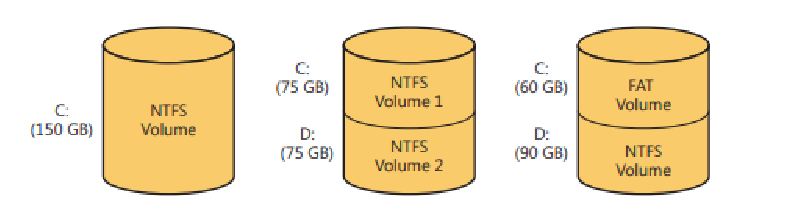
\includegraphics[scale=1]{dcd.eps}
\end{figure}

\subsection{IFS}
Windows uses IFS (Installable File System) as a file system API. By using an API the file systems do not have to be written to the kernel but can be instead by implemented as file system drivers, this means that file system developers can simply write a driver to add their file system to the operating system. This has some further advantages, such as not requiring applications to account for different file systems when trying to read or write data. They simply interact with IFS which then performs the appropriate operation with the file system driver.\cite{ifs}

Linux handles file systems in a very similar way using the VFS (Virtual File System). The virtual file system allows system calls such as read() and write() to be used regardless of the underlying file systems. For example if an application requests to write data, the VFS accepts the request and then requests the specific file system to write, at this point the file system handles actually writing the data.\cite{linux}

\lstset{language=C,caption={Registering a file system in Linux.\cite{code6}},label=code6}
\begin{lstlisting}[language=C]
int register_filesystem(struct file_system_type * fs)
{
	int res = 0;
	struct file_system_type ** p;

	BUG_ON(strchr(fs->name, '.'));
	if (fs->next)
		return -EBUSY;
	write_lock(&file_systems_lock);
	p = find_filesystem(fs->name, strlen(fs->name));
	if (*p)
		res = -EBUSY;
	else
		*p = fs;
	write_unlock(&file_systems_lock);
	return res;
}
\end{lstlisting}

\section{FreeBSD and Linux File systems and VFS comparison}

\subsection{ZFS}

In newer versions of FreeBSD ZFS is available as a native file system. ZFS is known as the zeta-byte file system as it can scale to zeta-byte sizes. The incredible scalability of the ZFS is one of its most appealing features. ZFS uses storage pools, these pools allow you to combine devices into a single pool which shares the disk space of all devices in the pool with all file systems in
the pool, another advantage of such a system is if you are running out of disk space you can simply add a new device to the pool to increase the available space. ZFS also features self-healing data, when a user is idle ZFS will use checksums to look for any possible failures. If a failure is found ZFS keeps redundant copies of data which it uses to repair the failure.\cite{zfs, linuxfs}

Due to incompatible open source licenses ZFS can not be included in the Linux kernel, though it is still possible to install ZFS support on a Linux system.\cite{linuxfs}

\subsection{ReiserFS}

FreeBSD supports read-only use of the Reiser file system. The Reiser file system has become less popular in recent years most likely due to the creator Han Reiser murdering his wife and being sent to prison.\cite{reiserfreebsd}

ReiserFS was once a native file system for some distributions of Linux, but has been primarily replaced by Ext4.\cite{reisermurder, linuxfs}

\subsection{UFS2}

UFS2 is FreeBSD's native file system, it is known as the Unix file system or the Berkeley Fast File System. Like Linux's Ext4 file systems it offers journaling, which allows it to repair inconsistencies that occur due to an unexpected shutdown of the system. What sets it apart from Ext4 is that it uses a special gjournal method that is block based and that is implemented through a GEOM extension. It also differs from Ext4 in that Ext4 offers a checksum for its journaling while UFS2 does not offer any form of checksum for its journaling.\cite{checksum, BSD, linux}

When comparing UFS2 to Linux's Ext4 they share a lot in common. They both have 255 byte file name limits. Both allow any characters in a file name with the exception of  NULL or "/" characters. Both have no path length limit (though their operating systems will enforce a limit), both support journaling, and both support sparse files.\cite{BSD, salter,linux}

\subsection{VFS}

Just like Linux, FreeBSD uses a VFS to help reduce the complexity of working with multiple and varying file systems. Both Linux and VFS allow applications to communicate with the VFS when requesting file system operations, then the VFS handles all communication with the the current file system using the correct method for that specific file system. This means that applications never need to know what file systems they are trying to interact with, the VFS acts as the mediator between the user space applications and the file system.\cite{linux, BSD}

\begin{figure}[H]
	\caption{The flow of data from user-space issuing a write() call, through the
VFS’s generic system call, into the filesystem’s specific write method, and finally arriving at the physical media.\cite{linux}}
  	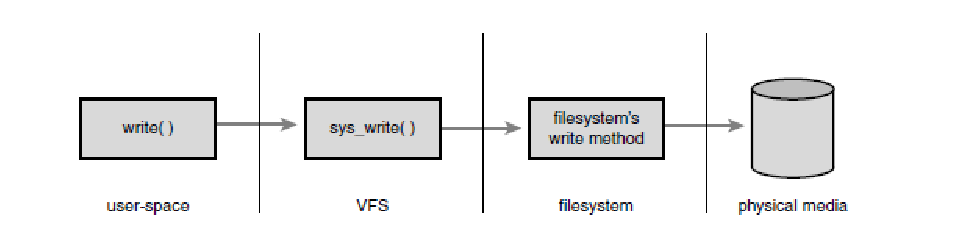
\includegraphics[scale=1]{vfsd.eps}
\end{figure}

Both Linux and FreeBSD use object oriented VFS to handle specific components of a file system.\cite{linux, BSD}

\subsubsection{Superblock} 
One such object is called a superblock. The superblock stores meta data and information that describes a given file system.\cite{linux, BSD} 

\subsubsection{File}
The file object is what processes interact with. It represents an open file and is created by the open() system call.\cite{linux, BSD}

\subsubsection{Inode}
The inode object contains meta-data to manipulate a file. Inodes represent a file in the file system with an inode number (this includes directories).\cite{linux, BSD}

\lstset{language=C,caption={Struct that makes up an inode in FreeBSD.\cite{code7}},label=code7}
\begin{lstlisting}[language=C]
struct inode {
	TAILQ_ENTRY(inode) i_nextsnap; /* snapshot file list. */
	struct	vnode  *i_vnode;/* Vnode associated with this inode. */
	struct 	ufsmount *i_ump;/* Ufsmount point associated with this inode. */
	struct	 dquot *i_dquot[MAXQUOTAS]; /* Dquot structures. */
	union {
		struct dirhash *dirhash; /* Hashing for large directories. */
		daddr_t *snapblklist;    /* Collect expunged snapshot blocks. */
	} i_un;
	/*
	 * The real copy of the on-disk inode.
	 */
	union {
		struct ufs1_dinode *din1;	/* UFS1 on-disk dinode. */
		struct ufs2_dinode *din2;	/* UFS2 on-disk dinode. */
	} dinode_u;

	ino_t	  i_number;	/* The identity of the inode. */
	u_int32_t i_flag;	/* flags, see below */
	int	  i_effnlink;	/* i_nlink when I/O completes */
\end{lstlisting}

\newpage

\section{Conclusion}

After exploring some of the features of Windows, FreeBSD, and Linux operating systems it is difficult not to have an appreciation for the incredible functionality provided transparently to the user. We have seen that FreeBSD and Linux share much of their design as they are both Unix-like operating systems, yet FreeBSD holds close to its Unix roots, letting us see how the two operating systems have diverged. Meanwhile Windows has some innovations all of its own, though we still find that it shares much in common with FreeBSD and Linux. We have explored I/O, processes, file systems, and many other topics. No one operating system stands above the rest, each has their own advantages that comes with unique trade offs. Leaving the users to decide what features they value.

\newpage

\bibliography{./WrtBib}
\bibliographystyle{IEEEtran}

\end{document}